\documentclass[11pt]{ctexart}
\usepackage[a4paper,margin=1in]{geometry}
\usepackage{longtable,booktabs,array}
\usepackage{xcolor}
\usepackage{listings}
\usepackage{hyperref}
\usepackage{pgfplots}
\pgfplotsset{compat=1.18}
\lstset{basicstyle=\ttfamily\small,breaklines=true,columns=fullflexible,showstringspaces=false}
\title{Geant4-Agent Full Test Report with Fuzzy-Language Robustness}
\author{Automated Evaluation Pipeline}
\date{2026-03-05}
\begin{document}
\maketitle
\section{Run Config}
\begin{itemize}
\item config: \texttt{nlu/bert\_lab/configs/deepseek\_api.local.json}
\item provider: \texttt{deepseek}
\item base\_url: \texttt{https://api.deepseek.com}
\item model: \texttt{deepseek-chat}
\item lang: \texttt{zh}, min\_confidence=0.6
\end{itemize}
\section{Summary Metrics}
\begin{longtable}{ll}
\toprule
metric & value\\
\midrule
total\_scenarios & 17.0000 \\
strict\_pass\_rate & 0.8235 \\
avg\_accuracy & 0.9069 \\
avg\_naturalness & 1.0000 \\
avg\_grounding\_mismatch\_rate & 0.0000 \\
closure\_rate & 0.8824 \\
avg\_turns\_per\_scenario & 1.6471 \\
clarification\_turn\_ratio & 0.3929 \\
overwrite\_guard\_pass\_rate & 1.0000 \\
contradiction\_detect\_rate & 1.0000 \\
fuzzy\_pass\_rate & 0.7778 \\
fuzzy\_closure\_rate & 0.7778 \\
failed\_ids & S08, F01, F07 \\
\bottomrule
\end{longtable}
\section{Scenario Table}
\begin{longtable}{p{0.08\linewidth}p{0.15\linewidth}p{0.22\linewidth}p{0.09\linewidth}p{0.10\linewidth}p{0.10\linewidth}p{0.12\linewidth}}
\toprule
id & category & domain & turns & accuracy & closure & pass \\
\midrule
S01 & full\_closure & Geometry+Source+Physics+Output & 1 & 1.000 & True & True \\
S02 & geometry\_family & Geometry family & 2 & 1.000 & True & True \\
S03 & overwrite\_control & Overwrite safety & 3 & 1.000 & True & True \\
S04 & question\_safety & Question turn behavior & 2 & 1.000 & True & True \\
S05 & source\_mode & Source mode & 1 & 1.000 & True & True \\
S06 & source\_mode & Source mode & 1 & 1.000 & True & True \\
S07 & consultative & Consultative flow & 2 & 1.000 & True & True \\
S08 & output\_update & Output update & 2 & 0.667 & True & False \\
F01 & fuzzy\_language & Fuzzy language & 2 & 0.750 & True & False \\
F02 & fuzzy\_language & Fuzzy language & 1 & 1.000 & True & True \\
F03 & fuzzy\_contradiction & Contradiction handling & 2 & 1.000 & True & True \\
F04 & fuzzy\_question & Question safety & 2 & 1.000 & True & True \\
F05 & fuzzy\_incomplete & Novice request & 1 & 1.000 & False & True \\
F06 & fuzzy\_units & Unit ambiguity & 1 & 1.000 & True & True \\
F07 & fuzzy\_output & Output update & 2 & 0.000 & True & False \\
F08 & fuzzy\_consultative & Consultative flow & 2 & 1.000 & True & True \\
F09 & fuzzy\_multimodal\_stub & Pseudo multimodal text & 1 & 1.000 & False & True \\
\bottomrule
\end{longtable}
\section{Category Table}
\begin{longtable}{p{0.08\linewidth}p{0.22\linewidth}p{0.10\linewidth}p{0.13\linewidth}p{0.13\linewidth}p{0.13\linewidth}p{0.13\linewidth}}
\toprule
legend & category & n & pass\_rate & closure\_rate & avg\_acc & avg\_nat \\
\midrule
C01 & consultative & 1 & 1.000 & 1.000 & 1.000 & 1.000 \\
C02 & full\_closure & 1 & 1.000 & 1.000 & 1.000 & 1.000 \\
C03 & fuzzy\_consultative & 1 & 1.000 & 1.000 & 1.000 & 1.000 \\
C04 & fuzzy\_contradiction & 1 & 1.000 & 1.000 & 1.000 & 1.000 \\
C05 & fuzzy\_incomplete & 1 & 1.000 & 0.000 & 1.000 & 1.000 \\
C06 & fuzzy\_language & 2 & 0.500 & 1.000 & 0.875 & 1.000 \\
C07 & fuzzy\_multimodal\_stub & 1 & 1.000 & 0.000 & 1.000 & 1.000 \\
C08 & fuzzy\_output & 1 & 0.000 & 1.000 & 0.000 & 1.000 \\
C09 & fuzzy\_question & 1 & 1.000 & 1.000 & 1.000 & 1.000 \\
C10 & fuzzy\_units & 1 & 1.000 & 1.000 & 1.000 & 1.000 \\
C11 & geometry\_family & 1 & 1.000 & 1.000 & 1.000 & 1.000 \\
C12 & output\_update & 1 & 0.000 & 1.000 & 0.667 & 1.000 \\
C13 & overwrite\_control & 1 & 1.000 & 1.000 & 1.000 & 1.000 \\
C14 & question\_safety & 1 & 1.000 & 1.000 & 1.000 & 1.000 \\
C15 & source\_mode & 2 & 1.000 & 1.000 & 1.000 & 1.000 \\
\bottomrule
\end{longtable}
\section{Visual Analysis}
\subsection{Scenario Accuracy}
\begin{center}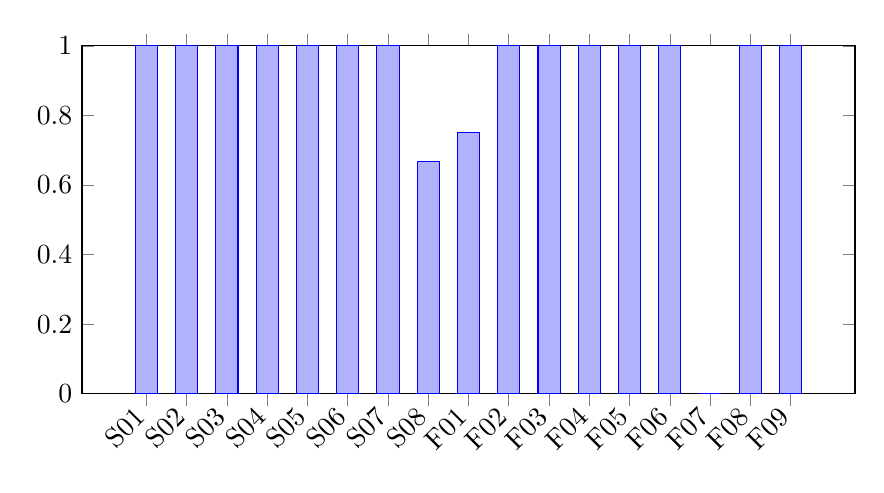
\begin{tikzpicture}
\begin{axis}[ybar,width=0.94\linewidth,height=6.0cm,ymin=0,ymax=1,symbolic x coords={S01,S02,S03,S04,S05,S06,S07,S08,F01,F02,F03,F04,F05,F06,F07,F08,F09},xtick=data,x tick label style={rotate=45,anchor=east},bar width=8pt]
\addplot coordinates {(S01,1.0000) (S02,1.0000) (S03,1.0000) (S04,1.0000) (S05,1.0000) (S06,1.0000) (S07,1.0000) (S08,0.6667) (F01,0.7500) (F02,1.0000) (F03,1.0000) (F04,1.0000) (F05,1.0000) (F06,1.0000) (F07,0.0000) (F08,1.0000) (F09,1.0000)};
\end{axis}\end{tikzpicture}\end{center}
\subsection{Scenario Naturalness}
\begin{center}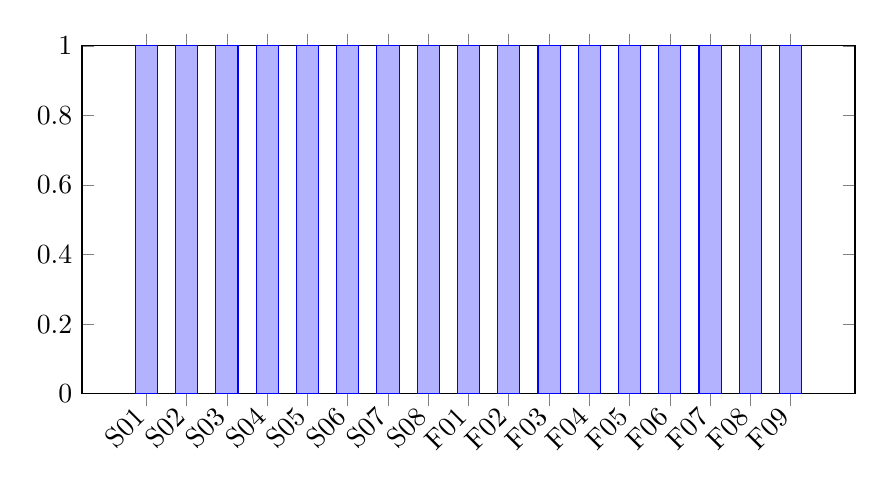
\begin{tikzpicture}
\begin{axis}[ybar,width=0.94\linewidth,height=6.0cm,ymin=0,ymax=1,symbolic x coords={S01,S02,S03,S04,S05,S06,S07,S08,F01,F02,F03,F04,F05,F06,F07,F08,F09},xtick=data,x tick label style={rotate=45,anchor=east},bar width=8pt]
\addplot coordinates {(S01,1.0000) (S02,1.0000) (S03,1.0000) (S04,1.0000) (S05,1.0000) (S06,1.0000) (S07,1.0000) (S08,1.0000) (F01,1.0000) (F02,1.0000) (F03,1.0000) (F04,1.0000) (F05,1.0000) (F06,1.0000) (F07,1.0000) (F08,1.0000) (F09,1.0000)};
\end{axis}\end{tikzpicture}\end{center}
\subsection{Category Pass vs Closure}
\begin{center}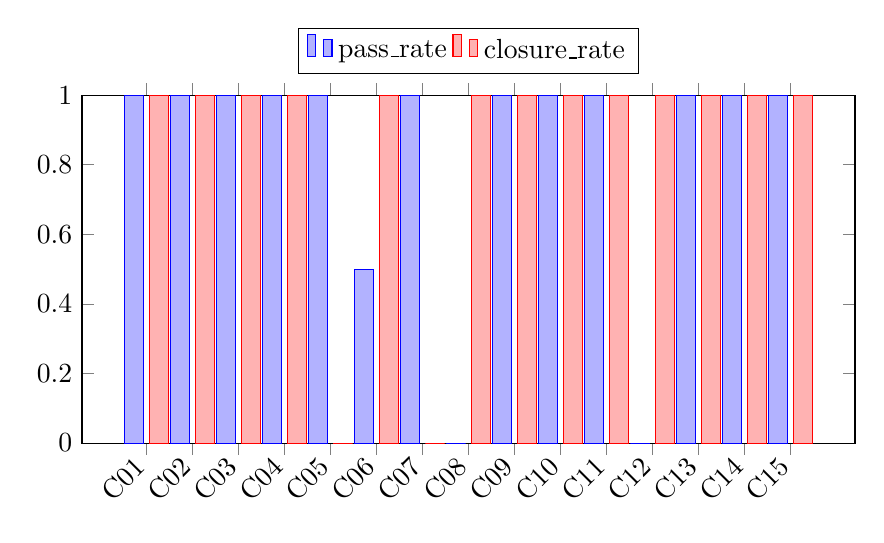
\begin{tikzpicture}
\begin{axis}[ybar,width=0.94\linewidth,height=6.0cm,ymin=0,ymax=1,symbolic x coords={C01,C02,C03,C04,C05,C06,C07,C08,C09,C10,C11,C12,C13,C14,C15},xtick=data,x tick label style={rotate=45,anchor=east},bar width=7pt,legend style={at={(0.5,1.06)},anchor=south,legend columns=2}]
\addplot coordinates {(C01,1.0000) (C02,1.0000) (C03,1.0000) (C04,1.0000) (C05,1.0000) (C06,0.5000) (C07,1.0000) (C08,0.0000) (C09,1.0000) (C10,1.0000) (C11,1.0000) (C12,0.0000) (C13,1.0000) (C14,1.0000) (C15,1.0000)};
\addplot coordinates {(C01,1.0000) (C02,1.0000) (C03,1.0000) (C04,1.0000) (C05,0.0000) (C06,1.0000) (C07,0.0000) (C08,1.0000) (C09,1.0000) (C10,1.0000) (C11,1.0000) (C12,1.0000) (C13,1.0000) (C14,1.0000) (C15,1.0000)};
\legend{pass\_rate,closure\_rate}
\end{axis}\end{tikzpicture}\end{center}
\section{Representative Raw Dialogues (1 per category)}
\subsection{consultative / S07: Consult then commit}
\paragraph{User-facing raw dialogue}
\begin{lstlisting}
[
  {
    "role": "user",
    "content": "This is pure gamma attenuation in copper, no hadrons. Recommend a Geant4 physics list and explain briefly."
  },
  {
    "role": "assistant",
    "content": "当前已提交配置为：物理列表 FTFP_BERT，输出格式 未指定，源类型 未指定，粒子 gamma。如需修改，请直接说明要改哪一项。"
  },
  {
    "role": "user",
    "content": "Adopt your recommendation. Geometry is 1m copper cube, gamma point 1MeV at center along +z, output json."
  },
  {
    "role": "assistant",
    "content": "好的，配置已经全部完成。根据您的设定，我们创建了一个边长为1米的铜立方体几何结构，并在其中心放置了一个沿+Z方向发射的1MeV伽马点源，输出格式为JSON。所有参数均已确认。"
  }
]
\end{lstlisting}
\paragraph{Internal iterative trace}
\begin{lstlisting}
[
  {
    "turn": 1,
    "user": "This is pure gamma attenuation in copper, no hadrons. Recommend a Geant4 physics list and explain briefly.",
    "assistant": "当前已提交配置为：物理列表 FTFP_BERT，输出格式 未指定，源类型 未指定，粒子 gamma。如需修改，请直接说明要改哪一项。",
    "dialogue_action": "summarize_progress",
    "asked_fields_friendly": [
      "几何结构类型",
      "几何参数 module_x"
    ],
    "missing_fields": [
      "geometry.structure",
      "geometry.params.module_x",
      "geometry.params.module_y",
      "geometry.params.module_z",
      "materials.volume_material_map",
      "source.type",
      "source.energy",
      "source.position",
      "source.direction",
      "output.format",
      "output.path"
    ],
    "normalization": {
      "intent": "SET",
      "confidence": 1.0,
      "backend": "llm_slot_frame"
    },
    "llm_used": true,
    "fallback_reason": null,
    "llm_stage_failures": [],
    "rejected_updates": [],
    "applied_rules": [
      {
        "path": "materials.selected_materials",
        "rule": "winner_selected",
        "producer": "slot_mapper",
        "confidence": 1.0
      },
      {
        "path": "source.particle",
        "rule": "winner_selected",
        "producer": "slot_mapper",
        "confidence": 1.0
      },
      {
        "path": "physics.physics_list",
        "rule": "winner_selected",
        "producer": "llm_recommender",
        "confidence": 0.95
      },
      {
        "path": "physics.backup_physics_list",
        "rule": "winner_selected",
        "producer": "llm_recommender",
        "confidence": 0.95
      },
      {
        "path": "physics.selection_reasons",
        "rule": "winner_selected",
        "producer": "llm_recommender",
        "confidence": 0.95
      },
      {
        "path": "physics.covered_processes",
        "rule": "winner_selected",
        "producer": "llm_recommender",
        "confidence": 0.95
      },
      {
        "path": "physics.selection_source",
        "rule": "winner_selected",
        "producer": "llm_recommender",
        "confidence": 0.95
      },
      {
        "rule": "post_commit_semantic_sync",
        "count": 4
      }
    ],
    "grounding_mismatch": false
  },
  {
    "turn": 2,
    "user": "Adopt your recommendation. Geometry is 1m copper cube, gamma point 1MeV at center along +z, output json.",
    "assistant": "好的，配置已经全部完成。根据您的设定，我们创建了一个边长为1米的铜立方体几何结构，并在其中心放置了一个沿+Z方向发射的1MeV伽马点源，输出格式为JSON。所有参数均已确认。",
    "dialogue_action": "finalize",
    "asked_fields_friendly": [],
    "missing_fields": [],
    "normalization": {
      "intent": "SET",
      "confidence": 1.0,
      "backend": "llm_slot_frame"
    },
    "llm_used": true,
    "fallback_reason": null,
    "llm_stage_failures": [],
    "rejected_updates": [
      {
        "path": "materials.selected_materials",
        "producer": "slot_mapper",
        "reason_code": "E_LOCKED_FIELD_OVERRIDE",
        "detail": "attempt to modify locked field"
      },
      {
        "path": "source.particle",
        "producer": "slot_mapper",
        "reason_code": "E_LOCKED_FIELD_OVERRIDE",
        "detail": "attempt to modify locked field"
      },
      {
        "path": "output.format",
        "producer": "slot_mapper",
        "reason_code": "E_LOWER_PRIORITY",
        "detail": "superseded by winner"
      }
    ],
    "applied_rules": [
      {
        "path": "geometry.structure",
        "rule": "winner_selected",
        "producer": "slot_mapper",
        "confidence": 1.0
      },
      {
        "path": "geometry.params.module_x",
        "rule": "winner_selected",
        "producer": "slot_mapper",
        "confidence": 1.0
      },
      {
        "path": "geometry.params.module_y",
        "rule": "winner_selected",
        "producer": "slot_mapper",
        "confidence": 1.0
      },
      {
        "path": "geometry.params.module_z",
        "rule": "winner_selected",
        "producer": "slot_mapper",
        "confidence": 1.0
      },
      {
        "path": "source.type",
        "rule": "winner_selected",
        "producer": "slot_mapper",
        "confidence": 1.0
      },
      {
        "path": "source.energy",
        "rule": "winner_selected",
        "producer": "slot_mapper",
        "confidence": 1.0
      },
      {
        "path": "source.position",
        "rule": "winner_selected",
        "producer": "slot_mapper",
        "confidence": 1.0
      },
      {
        "path": "source.direction",
        "rule": "winner_selected",
        "producer": "slot_mapper",
        "confidence": 1.0
      }
    ],
    "grounding_mismatch": false
  }
]
\end{lstlisting}
\paragraph{Checks}
\begin{lstlisting}
[
  {
    "field": "complete",
    "expected": true,
    "actual": true,
    "ok": true
  },
  {
    "field": "physics.physics_list",
    "expected": "FTFP_BERT",
    "actual": "FTFP_BERT",
    "ok": true
  },
  {
    "field": "output.format",
    "expected": "json",
    "actual": "json",
    "ok": true
  }
]
\end{lstlisting}
\subsection{full\_closure / S01: Single-turn full closure}
\paragraph{User-facing raw dialogue}
\begin{lstlisting}
[
  {
    "role": "user",
    "content": "Need a 1m x 1m x 1m copper box, gamma point source 1 MeV at center along +z, physics FTFP_BERT, output json."
  },
  {
    "role": "assistant",
    "content": "配置已完成。"
  }
]
\end{lstlisting}
\paragraph{Internal iterative trace}
\begin{lstlisting}
[
  {
    "turn": 1,
    "user": "Need a 1m x 1m x 1m copper box, gamma point source 1 MeV at center along +z, physics FTFP_BERT, output json.",
    "assistant": "配置已完成。",
    "dialogue_action": "finalize",
    "asked_fields_friendly": [],
    "missing_fields": [],
    "normalization": {
      "intent": "SET",
      "confidence": 1.0,
      "backend": "llm_slot_frame"
    },
    "llm_used": true,
    "fallback_reason": null,
    "llm_stage_failures": [],
    "rejected_updates": [
      {
        "path": "physics.physics_list",
        "producer": "slot_mapper",
        "reason_code": "E_LOWER_PRIORITY",
        "detail": "superseded by winner"
      },
      {
        "path": "output.format",
        "producer": "slot_mapper",
        "reason_code": "E_LOWER_PRIORITY",
        "detail": "superseded by winner"
      }
    ],
    "applied_rules": [
      {
        "path": "geometry.structure",
        "rule": "winner_selected",
        "producer": "slot_mapper",
        "confidence": 1.0
      },
      {
        "path": "geometry.params.module_x",
        "rule": "winner_selected",
        "producer": "slot_mapper",
        "confidence": 1.0
      },
      {
        "path": "geometry.params.module_y",
        "rule": "winner_selected",
        "producer": "slot_mapper",
        "confidence": 1.0
      },
      {
        "path": "geometry.params.module_z",
        "rule": "winner_selected",
        "producer": "slot_mapper",
        "confidence": 1.0
      },
      {
        "path": "materials.selected_materials",
        "rule": "winner_selected",
        "producer": "slot_mapper",
        "confidence": 1.0
      },
      {
        "path": "source.type",
        "rule": "winner_selected",
        "producer": "slot_mapper",
        "confidence": 1.0
      },
      {
        "path": "source.particle",
        "rule": "winner_selected",
        "producer": "slot_mapper",
        "confidence": 1.0
      },
      {
        "path": "source.energy",
        "rule": "winner_selected",
        "producer": "slot_mapper",
        "confidence": 1.0
      }
    ],
    "grounding_mismatch": false
  }
]
\end{lstlisting}
\paragraph{Checks}
\begin{lstlisting}
[
  {
    "field": "complete",
    "expected": true,
    "actual": true,
    "ok": true
  },
  {
    "field": "geometry.structure",
    "expected": "single_box",
    "actual": "single_box",
    "ok": true
  },
  {
    "field": "source.type",
    "expected": "point",
    "actual": "point",
    "ok": true
  },
  {
    "field": "source.particle",
    "expected": "gamma",
    "actual": "gamma",
    "ok": true
  },
  {
    "field": "physics.physics_list",
    "expected": "FTFP_BERT",
    "actual": "FTFP_BERT",
    "ok": true
  },
  {
    "field": "output.format",
    "expected": "json",
    "actual": "json",
    "ok": true
  }
]
\end{lstlisting}
\subsection{fuzzy\_consultative / F08: Consultative with fuzzy wording}
\paragraph{User-facing raw dialogue}
\begin{lstlisting}
[
  {
    "role": "user",
    "content": "I only care about gamma attenuation in copper and no hadrons. Recommend a safe Geant4 physics list."
  },
  {
    "role": "assistant",
    "content": "好的，当前配置进度如下：\n\n**已完成：**\n*   **材料**：已选定铜。\n*   **源**：已确定粒子类型为伽马射线。\n*   **物理**：已根据您的要求（仅关心伽马在铜中的衰减，无需强子物理），推荐并设置了安全的物理列表。\n\n**待补充：**\n*   **几何**：需要您提供探测器的几何结构类型和具体尺寸。\n*   **材料绑定**：需要明确将铜材料具体绑定到哪个几何体积上。\n*   **源细节**：需要设定源的类型（如点源、面源等）和能量。\n*   **输出**：需要指定输出数据的格式和保存路径。\n\n请先补充几何结构的相关信息。"
  },
  {
    "role": "user",
    "content": "Use your recommendation. Geometry 1m copper cube, gamma point 1MeV at center +z, output json."
  },
  {
    "role": "assistant",
    "content": "好的，配置已经全部完成！\n\n根据您最新的要求，我已为您整合并确认了以下设置：\n*   **几何**：一个边长为1米的铜立方体。\n*   **源**：中心位置、沿+Z方向发射的1MeV伽马点源。\n*   **物理**：采用推荐的、安全的物理列表（仅包含伽马相关过程）。\n*   **输出**：结果将保存为JSON格式。\n\n所有参数均已就绪，可以开始运行模拟了。"
  }
]
\end{lstlisting}
\paragraph{Internal iterative trace}
\begin{lstlisting}
[
  {
    "turn": 1,
    "user": "I only care about gamma attenuation in copper and no hadrons. Recommend a safe Geant4 physics list.",
    "assistant": "好的，当前配置进度如下：\n\n**已完成：**\n*   **材料**：已选定铜。\n*   **源**：已确定粒子类型为伽马射线。\n*   **物理**：已根据您的要求（仅关心伽马在铜中的衰减，无需强子物理），推荐并设置了安全的物理列表。\n\n**待补充：**\n*   **几何**：需要您提供探测器的几何结构类型和具体尺寸。\n*   **材料绑定**：需要明确将铜材料具体绑定到哪个几何体积上。\n*   **源细节**：需要设定源的类型（如点源、面源等）和能量。\n*   **输出**：需要指定输出数据的格式和保存路径。\n\n请先补充几何结构的相关信息。",
    "dialogue_action": "summarize_progress",
    "asked_fields_friendly": [
      "几何结构类型",
      "几何参数 module_x"
    ],
    "missing_fields": [
      "geometry.structure",
      "geometry.params.module_x",
      "geometry.params.module_y",
      "geometry.params.module_z",
      "materials.volume_material_map",
      "source.type",
      "source.energy",
      "source.position",
      "source.direction",
      "output.format",
      "output.path"
    ],
    "normalization": {
      "intent": "MODIFY",
      "confidence": 0.95,
      "backend": "llm_slot_frame"
    },
    "llm_used": true,
    "fallback_reason": null,
    "llm_stage_failures": [],
    "rejected_updates": [],
    "applied_rules": [
      {
        "path": "materials.selected_materials",
        "rule": "winner_selected",
        "producer": "slot_mapper",
        "confidence": 0.95
      },
      {
        "path": "source.particle",
        "rule": "winner_selected",
        "producer": "slot_mapper",
        "confidence": 0.95
      },
      {
        "path": "physics.physics_list",
        "rule": "winner_selected",
        "producer": "llm_recommender",
        "confidence": 0.95
      },
      {
        "path": "physics.backup_physics_list",
        "rule": "winner_selected",
        "producer": "llm_recommender",
        "confidence": 0.95
      },
      {
        "path": "physics.selection_reasons",
        "rule": "winner_selected",
        "producer": "llm_recommender",
        "confidence": 0.95
      },
      {
        "path": "physics.covered_processes",
        "rule": "winner_selected",
        "producer": "llm_recommender",
        "confidence": 0.95
      },
      {
        "path": "physics.selection_source",
        "rule": "winner_selected",
        "producer": "llm_recommender",
        "confidence": 0.95
      },
      {
        "rule": "post_commit_semantic_sync",
        "count": 4
      }
    ],
    "grounding_mismatch": false
  },
  {
    "turn": 2,
    "user": "Use your recommendation. Geometry 1m copper cube, gamma point 1MeV at center +z, output json.",
    "assistant": "好的，配置已经全部完成！\n\n根据您最新的要求，我已为您整合并确认了以下设置：\n*   **几何**：一个边长为1米的铜立方体。\n*   **源**：中心位置、沿+Z方向发射的1MeV伽马点源。\n*   **物理**：采用推荐的、安全的物理列表（仅包含伽马相关过程）。\n*   **输出**：结果将保存为JSON格式。\n\n所有参数均已就绪，可以开始运行模拟了。",
    "dialogue_action": "finalize",
    "asked_fields_friendly": [],
    "missing_fields": [],
    "normalization": {
      "intent": "SET",
      "confidence": 1.0,
      "backend": "llm_slot_frame"
    },
    "llm_used": true,
    "fallback_reason": null,
    "llm_stage_failures": [],
    "rejected_updates": [
      {
        "path": "materials.selected_materials",
        "producer": "slot_mapper",
        "reason_code": "E_LOCKED_FIELD_OVERRIDE",
        "detail": "attempt to modify locked field"
      },
      {
        "path": "source.particle",
        "producer": "slot_mapper",
        "reason_code": "E_LOCKED_FIELD_OVERRIDE",
        "detail": "attempt to modify locked field"
      },
      {
        "path": "output.format",
        "producer": "slot_mapper",
        "reason_code": "E_LOWER_PRIORITY",
        "detail": "superseded by winner"
      }
    ],
    "applied_rules": [
      {
        "path": "geometry.structure",
        "rule": "winner_selected",
        "producer": "slot_mapper",
        "confidence": 1.0
      },
      {
        "path": "geometry.params.module_x",
        "rule": "winner_selected",
        "producer": "slot_mapper",
        "confidence": 1.0
      },
      {
        "path": "geometry.params.module_y",
        "rule": "winner_selected",
        "producer": "slot_mapper",
        "confidence": 1.0
      },
      {
        "path": "geometry.params.module_z",
        "rule": "winner_selected",
        "producer": "slot_mapper",
        "confidence": 1.0
      },
      {
        "path": "source.type",
        "rule": "winner_selected",
        "producer": "slot_mapper",
        "confidence": 1.0
      },
      {
        "path": "source.energy",
        "rule": "winner_selected",
        "producer": "slot_mapper",
        "confidence": 1.0
      },
      {
        "path": "source.position",
        "rule": "winner_selected",
        "producer": "slot_mapper",
        "confidence": 1.0
      },
      {
        "path": "source.direction",
        "rule": "winner_selected",
        "producer": "slot_mapper",
        "confidence": 1.0
      }
    ],
    "grounding_mismatch": false
  }
]
\end{lstlisting}
\paragraph{Checks}
\begin{lstlisting}
[
  {
    "field": "complete",
    "expected": true,
    "actual": true,
    "ok": true
  },
  {
    "field": "output.format",
    "expected": "json",
    "actual": "json",
    "ok": true
  }
]
\end{lstlisting}
\subsection{fuzzy\_contradiction / F03: Contradictory rewrite in one turn}
\paragraph{User-facing raw dialogue}
\begin{lstlisting}
[
  {
    "role": "user",
    "content": "Copper cube 1m x 1m x 1m, gamma point 1 MeV at center +z, physics FTFP_BERT, output json."
  },
  {
    "role": "assistant",
    "content": "好的，你的 Geant4 配置已经完成了！\n\n根据你提供的信息，我们已经设定了：\n*   **几何**：一个 1m x 1m x 1m 的立方体模块。\n*   **材料**：立方体材料为铜 (Copper)。\n*   **物理过程**：使用 FTFP_BERT 物理列表。\n*   **粒子源**：在中心位置，沿 +Z 方向发射 1 MeV 能量的伽马射线。\n*   **输出**：结果将保存为 JSON 格式。\n\n所有必要参数都已确认，可以准备运行模拟了。"
  },
  {
    "role": "user",
    "content": "Change geometry to cylinder radius 30mm, but keep the 1m cube unchanged."
  },
  {
    "role": "assistant",
    "content": "检测到要修改已确认的几何结构。请确认是否将几何结构类型从“立方体”改为“圆柱体”？"
  }
]
\end{lstlisting}
\paragraph{Internal iterative trace}
\begin{lstlisting}
[
  {
    "turn": 1,
    "user": "Copper cube 1m x 1m x 1m, gamma point 1 MeV at center +z, physics FTFP_BERT, output json.",
    "assistant": "好的，你的 Geant4 配置已经完成了！\n\n根据你提供的信息，我们已经设定了：\n*   **几何**：一个 1m x 1m x 1m 的立方体模块。\n*   **材料**：立方体材料为铜 (Copper)。\n*   **物理过程**：使用 FTFP_BERT 物理列表。\n*   **粒子源**：在中心位置，沿 +Z 方向发射 1 MeV 能量的伽马射线。\n*   **输出**：结果将保存为 JSON 格式。\n\n所有必要参数都已确认，可以准备运行模拟了。",
    "dialogue_action": "finalize",
    "asked_fields_friendly": [],
    "missing_fields": [],
    "normalization": {
      "intent": "SET",
      "confidence": 1.0,
      "backend": "llm_slot_frame"
    },
    "llm_used": true,
    "fallback_reason": null,
    "llm_stage_failures": [],
    "rejected_updates": [
      {
        "path": "physics.physics_list",
        "producer": "slot_mapper",
        "reason_code": "E_LOWER_PRIORITY",
        "detail": "superseded by winner"
      },
      {
        "path": "output.format",
        "producer": "slot_mapper",
        "reason_code": "E_LOWER_PRIORITY",
        "detail": "superseded by winner"
      }
    ],
    "applied_rules": [
      {
        "path": "geometry.structure",
        "rule": "winner_selected",
        "producer": "slot_mapper",
        "confidence": 1.0
      },
      {
        "path": "geometry.params.module_x",
        "rule": "winner_selected",
        "producer": "slot_mapper",
        "confidence": 1.0
      },
      {
        "path": "geometry.params.module_y",
        "rule": "winner_selected",
        "producer": "slot_mapper",
        "confidence": 1.0
      },
      {
        "path": "geometry.params.module_z",
        "rule": "winner_selected",
        "producer": "slot_mapper",
        "confidence": 1.0
      },
      {
        "path": "materials.selected_materials",
        "rule": "winner_selected",
        "producer": "slot_mapper",
        "confidence": 1.0
      },
      {
        "path": "source.type",
        "rule": "winner_selected",
        "producer": "slot_mapper",
        "confidence": 1.0
      },
      {
        "path": "source.particle",
        "rule": "winner_selected",
        "producer": "slot_mapper",
        "confidence": 1.0
      },
      {
        "path": "source.energy",
        "rule": "winner_selected",
        "producer": "slot_mapper",
        "confidence": 1.0
      }
    ],
    "grounding_mismatch": false
  },
  {
    "turn": 2,
    "user": "Change geometry to cylinder radius 30mm, but keep the 1m cube unchanged.",
    "assistant": "检测到要修改已确认的几何结构。请确认是否将几何结构类型从“立方体”改为“圆柱体”？",
    "dialogue_action": "confirm_overwrite",
    "asked_fields_friendly": [],
    "missing_fields": [],
    "normalization": {
      "intent": "MODIFY",
      "confidence": 0.95,
      "backend": "llm_slot_frame"
    },
    "llm_used": true,
    "fallback_reason": null,
    "llm_stage_failures": [],
    "rejected_updates": [
      {
        "path": "geometry.params.module_x",
        "producer": "slot_mapper",
        "reason_code": "E_LOCKED_FIELD_OVERRIDE",
        "detail": "attempt to modify locked field"
      },
      {
        "path": "geometry.params.module_y",
        "producer": "slot_mapper",
        "reason_code": "E_LOCKED_FIELD_OVERRIDE",
        "detail": "attempt to modify locked field"
      },
      {
        "path": "geometry.params.module_z",
        "producer": "slot_mapper",
        "reason_code": "E_LOCKED_FIELD_OVERRIDE",
        "detail": "attempt to modify locked field"
      }
    ],
    "applied_rules": [
      {
        "rule": "pending_overwrite_confirmation_required",
        "count": 1
      },
      {
        "path": "geometry.params.child_rmax",
        "rule": "winner_selected",
        "producer": "slot_mapper",
        "confidence": 0.95
      }
    ],
    "grounding_mismatch": false
  }
]
\end{lstlisting}
\paragraph{Checks}
\begin{lstlisting}
[
  {
    "field": "geometry.structure",
    "expected": "single_box",
    "actual": "single_box",
    "ok": true
  },
  {
    "field": "has_any_action",
    "expected": [
      "confirm_overwrite",
      "ask_clarification"
    ],
    "actual": [
      "confirm_overwrite"
    ],
    "ok": true
  }
]
\end{lstlisting}
\subsection{fuzzy\_incomplete / F05: Incomplete novice input}
\paragraph{User-facing raw dialogue}
\begin{lstlisting}
[
  {
    "role": "user",
    "content": "Can you set up a copper gamma test and give me a runnable baseline?"
  },
  {
    "role": "assistant",
    "content": "目前配置进度如下：\n\n**几何**：待补充结构类型和尺寸参数。  \n**材料**：已选定铜，并记录了选择依据和来源；待补充材料与体积的绑定关系。  \n**源**：已确定使用伽马射线，并记录了选择依据和来源；待补充具体的源类型和能量。  \n**物理**：待选择物理列表。  \n**输出**：待指定输出格式和保存路径。\n\n请继续补充待完善的信息，以便生成可运行的基线配置。"
  }
]
\end{lstlisting}
\paragraph{Internal iterative trace}
\begin{lstlisting}
[
  {
    "turn": 1,
    "user": "Can you set up a copper gamma test and give me a runnable baseline?",
    "assistant": "目前配置进度如下：\n\n**几何**：待补充结构类型和尺寸参数。  \n**材料**：已选定铜，并记录了选择依据和来源；待补充材料与体积的绑定关系。  \n**源**：已确定使用伽马射线，并记录了选择依据和来源；待补充具体的源类型和能量。  \n**物理**：待选择物理列表。  \n**输出**：待指定输出格式和保存路径。\n\n请继续补充待完善的信息，以便生成可运行的基线配置。",
    "dialogue_action": "summarize_progress",
    "asked_fields_friendly": [
      "几何结构类型",
      "几何参数 module_x"
    ],
    "missing_fields": [
      "geometry.structure",
      "geometry.params.module_x",
      "geometry.params.module_y",
      "geometry.params.module_z",
      "materials.volume_material_map",
      "source.type",
      "source.energy",
      "source.position",
      "source.direction",
      "physics.physics_list",
      "output.format",
      "output.path"
    ],
    "normalization": {
      "intent": "QUESTION",
      "confidence": 0.95,
      "backend": "llm_slot_frame"
    },
    "llm_used": true,
    "fallback_reason": null,
    "llm_stage_failures": [],
    "rejected_updates": [],
    "applied_rules": [
      {
        "path": "materials.selected_materials",
        "rule": "winner_selected",
        "producer": "slot_mapper",
        "confidence": 0.95
      },
      {
        "path": "source.particle",
        "rule": "winner_selected",
        "producer": "slot_mapper",
        "confidence": 0.95
      },
      {
        "rule": "post_commit_semantic_sync",
        "count": 4
      }
    ],
    "grounding_mismatch": false
  }
]
\end{lstlisting}
\paragraph{Checks}
\begin{lstlisting}
[
  {
    "field": "complete",
    "expected": false,
    "actual": false,
    "ok": true
  },
  {
    "field": "missing_at_least",
    "expected": 1,
    "actual": 12,
    "ok": true
  },
  {
    "field": "has_any_action",
    "expected": [
      "ask_clarification",
      "summarize_progress",
      "answer_status"
    ],
    "actual": [
      "summarize_progress"
    ],
    "ok": true
  }
]
\end{lstlisting}
\subsection{fuzzy\_language / F02: Code-switch shorthand}
\paragraph{User-facing raw dialogue}
\begin{lstlisting}
[
  {
    "role": "user",
    "content": "target: Cu cube 1000mm^3 each side; src gamma point E=1MeV pos(0,0,0) dir(0,0,1); physics=FTFP_BERT; output=root"
  },
  {
    "role": "assistant",
    "content": "配置已完成。"
  }
]
\end{lstlisting}
\paragraph{Internal iterative trace}
\begin{lstlisting}
[
  {
    "turn": 1,
    "user": "target: Cu cube 1000mm^3 each side; src gamma point E=1MeV pos(0,0,0) dir(0,0,1); physics=FTFP_BERT; output=root",
    "assistant": "配置已完成。",
    "dialogue_action": "finalize",
    "asked_fields_friendly": [],
    "missing_fields": [],
    "normalization": {
      "intent": "SET",
      "confidence": 1.0,
      "backend": "llm_slot_frame"
    },
    "llm_used": true,
    "fallback_reason": null,
    "llm_stage_failures": [],
    "rejected_updates": [
      {
        "path": "physics.physics_list",
        "producer": "slot_mapper",
        "reason_code": "E_LOWER_PRIORITY",
        "detail": "superseded by winner"
      },
      {
        "path": "output.format",
        "producer": "slot_mapper",
        "reason_code": "E_LOWER_PRIORITY",
        "detail": "superseded by winner"
      }
    ],
    "applied_rules": [
      {
        "path": "geometry.structure",
        "rule": "winner_selected",
        "producer": "slot_mapper",
        "confidence": 1.0
      },
      {
        "path": "geometry.params.module_x",
        "rule": "winner_selected",
        "producer": "slot_mapper",
        "confidence": 1.0
      },
      {
        "path": "geometry.params.module_y",
        "rule": "winner_selected",
        "producer": "slot_mapper",
        "confidence": 1.0
      },
      {
        "path": "geometry.params.module_z",
        "rule": "winner_selected",
        "producer": "slot_mapper",
        "confidence": 1.0
      },
      {
        "path": "materials.selected_materials",
        "rule": "winner_selected",
        "producer": "slot_mapper",
        "confidence": 1.0
      },
      {
        "path": "source.type",
        "rule": "winner_selected",
        "producer": "slot_mapper",
        "confidence": 1.0
      },
      {
        "path": "source.particle",
        "rule": "winner_selected",
        "producer": "slot_mapper",
        "confidence": 1.0
      },
      {
        "path": "source.energy",
        "rule": "winner_selected",
        "producer": "slot_mapper",
        "confidence": 1.0
      }
    ],
    "grounding_mismatch": false
  }
]
\end{lstlisting}
\paragraph{Checks}
\begin{lstlisting}
[
  {
    "field": "complete",
    "expected": true,
    "actual": true,
    "ok": true
  },
  {
    "field": "geometry.structure",
    "expected": "single_box",
    "actual": "single_box",
    "ok": true
  },
  {
    "field": "source.type",
    "expected": "point",
    "actual": "point",
    "ok": true
  },
  {
    "field": "output.format",
    "expected": "root",
    "actual": "root",
    "ok": true
  }
]
\end{lstlisting}
\subsection{fuzzy\_multimodal\_stub / F09: Multimodal placeholder text}
\paragraph{User-facing raw dialogue}
\begin{lstlisting}
[
  {
    "role": "user",
    "content": "Follow this sketch: [image: copper cube, center source, +z direction], build config first."
  },
  {
    "role": "assistant",
    "content": "当前配置进度如下：\n\n几何部分已设定好结构类型和X、Y方向尺寸；材料部分已选定具体材料并完成与体积的绑定；源部分已设定类型、能量和位置，还需补充粒子类型；物理列表以及输出格式、路径尚待补充。"
  }
]
\end{lstlisting}
\paragraph{Internal iterative trace}
\begin{lstlisting}
[
  {
    "turn": 1,
    "user": "Follow this sketch: [image: copper cube, center source, +z direction], build config first.",
    "assistant": "当前配置进度如下：\n\n几何部分已设定好结构类型和X、Y方向尺寸；材料部分已选定具体材料并完成与体积的绑定；源部分已设定类型、能量和位置，还需补充粒子类型；物理列表以及输出格式、路径尚待补充。",
    "dialogue_action": "summarize_progress",
    "asked_fields_friendly": [
      "粒子类型",
      "物理列表"
    ],
    "missing_fields": [
      "source.particle",
      "physics.physics_list",
      "output.format",
      "output.path"
    ],
    "normalization": {
      "intent": "SET",
      "confidence": 1.0,
      "backend": "llm_slot_frame"
    },
    "llm_used": true,
    "fallback_reason": null,
    "llm_stage_failures": [],
    "rejected_updates": [],
    "applied_rules": [
      {
        "path": "geometry.structure",
        "rule": "winner_selected",
        "producer": "slot_mapper",
        "confidence": 1.0
      },
      {
        "path": "geometry.params.module_x",
        "rule": "winner_selected",
        "producer": "slot_mapper",
        "confidence": 1.0
      },
      {
        "path": "geometry.params.module_y",
        "rule": "winner_selected",
        "producer": "slot_mapper",
        "confidence": 1.0
      },
      {
        "path": "geometry.params.module_z",
        "rule": "winner_selected",
        "producer": "slot_mapper",
        "confidence": 1.0
      },
      {
        "path": "materials.selected_materials",
        "rule": "winner_selected",
        "producer": "slot_mapper",
        "confidence": 1.0
      },
      {
        "path": "source.type",
        "rule": "winner_selected",
        "producer": "slot_mapper",
        "confidence": 1.0
      },
      {
        "path": "source.energy",
        "rule": "winner_selected",
        "producer": "slot_mapper",
        "confidence": 1.0
      },
      {
        "path": "source.position",
        "rule": "winner_selected",
        "producer": "slot_mapper",
        "confidence": 1.0
      }
    ],
    "grounding_mismatch": false
  }
]
\end{lstlisting}
\paragraph{Checks}
\begin{lstlisting}
[
  {
    "field": "complete",
    "expected": false,
    "actual": false,
    "ok": true
  },
  {
    "field": "missing_at_least",
    "expected": 1,
    "actual": 4,
    "ok": true
  },
  {
    "field": "has_any_action",
    "expected": [
      "ask_clarification",
      "answer_status",
      "summarize_progress"
    ],
    "actual": [
      "summarize_progress"
    ],
    "ok": true
  }
]
\end{lstlisting}
\subsection{fuzzy\_output / F07: Colloquial output rewrite}
\paragraph{User-facing raw dialogue}
\begin{lstlisting}
[
  {
    "role": "user",
    "content": "Copper cube 1m x 1m x 1m, gamma point 1 MeV at center +z, physics FTFP_BERT, output json."
  },
  {
    "role": "assistant",
    "content": "配置已完成。"
  },
  {
    "role": "user",
    "content": "I want the ROOT tree style output file."
  },
  {
    "role": "assistant",
    "content": "检测到您想要修改输出格式。请确认是否将输出格式从 json 改为 root？"
  }
]
\end{lstlisting}
\paragraph{Internal iterative trace}
\begin{lstlisting}
[
  {
    "turn": 1,
    "user": "Copper cube 1m x 1m x 1m, gamma point 1 MeV at center +z, physics FTFP_BERT, output json.",
    "assistant": "配置已完成。",
    "dialogue_action": "finalize",
    "asked_fields_friendly": [],
    "missing_fields": [],
    "normalization": {
      "intent": "SET",
      "confidence": 1.0,
      "backend": "llm_slot_frame"
    },
    "llm_used": true,
    "fallback_reason": null,
    "llm_stage_failures": [],
    "rejected_updates": [
      {
        "path": "physics.physics_list",
        "producer": "slot_mapper",
        "reason_code": "E_LOWER_PRIORITY",
        "detail": "superseded by winner"
      },
      {
        "path": "output.format",
        "producer": "slot_mapper",
        "reason_code": "E_LOWER_PRIORITY",
        "detail": "superseded by winner"
      }
    ],
    "applied_rules": [
      {
        "path": "geometry.structure",
        "rule": "winner_selected",
        "producer": "slot_mapper",
        "confidence": 1.0
      },
      {
        "path": "geometry.params.module_x",
        "rule": "winner_selected",
        "producer": "slot_mapper",
        "confidence": 1.0
      },
      {
        "path": "geometry.params.module_y",
        "rule": "winner_selected",
        "producer": "slot_mapper",
        "confidence": 1.0
      },
      {
        "path": "geometry.params.module_z",
        "rule": "winner_selected",
        "producer": "slot_mapper",
        "confidence": 1.0
      },
      {
        "path": "materials.selected_materials",
        "rule": "winner_selected",
        "producer": "slot_mapper",
        "confidence": 1.0
      },
      {
        "path": "source.type",
        "rule": "winner_selected",
        "producer": "slot_mapper",
        "confidence": 1.0
      },
      {
        "path": "source.particle",
        "rule": "winner_selected",
        "producer": "slot_mapper",
        "confidence": 1.0
      },
      {
        "path": "source.energy",
        "rule": "winner_selected",
        "producer": "slot_mapper",
        "confidence": 1.0
      }
    ],
    "grounding_mismatch": false
  },
  {
    "turn": 2,
    "user": "I want the ROOT tree style output file.",
    "assistant": "检测到您想要修改输出格式。请确认是否将输出格式从 json 改为 root？",
    "dialogue_action": "confirm_overwrite",
    "asked_fields_friendly": [],
    "missing_fields": [],
    "normalization": {
      "intent": "SET",
      "confidence": 1.0,
      "backend": "llm_slot_frame"
    },
    "llm_used": true,
    "fallback_reason": null,
    "llm_stage_failures": [],
    "rejected_updates": [],
    "applied_rules": [
      {
        "rule": "pending_overwrite_confirmation_required",
        "count": 1
      }
    ],
    "grounding_mismatch": false
  }
]
\end{lstlisting}
\paragraph{Checks}
\begin{lstlisting}
[
  {
    "field": "output.format",
    "expected": "root",
    "actual": "json",
    "ok": false
  }
]
\end{lstlisting}
\subsection{fuzzy\_question / F04: Fuzzy question should not overwrite}
\paragraph{User-facing raw dialogue}
\begin{lstlisting}
[
  {
    "role": "user",
    "content": "Setup 1m copper cube, gamma 1MeV point source at center +z, FTFP_BERT, json output."
  },
  {
    "role": "assistant",
    "content": "配置已完成，所有参数已根据你的输入设置完毕。"
  },
  {
    "role": "user",
    "content": "Would proton be better?"
  },
  {
    "role": "assistant",
    "content": "我为你解释一下当前配置的依据：\n\n**物理列表**：根据你明确指定的“FTFP_BERT”设置。\n**材料**：根据你明确提供的“1m copper cube”设置。\n**源**：根据你明确描述的“gamma 1MeV point source at center +z”设置。\n\n以上所有参数都已确认并生效。"
  }
]
\end{lstlisting}
\paragraph{Internal iterative trace}
\begin{lstlisting}
[
  {
    "turn": 1,
    "user": "Setup 1m copper cube, gamma 1MeV point source at center +z, FTFP_BERT, json output.",
    "assistant": "配置已完成，所有参数已根据你的输入设置完毕。",
    "dialogue_action": "finalize",
    "asked_fields_friendly": [],
    "missing_fields": [],
    "normalization": {
      "intent": "SET",
      "confidence": 1.0,
      "backend": "llm_slot_frame"
    },
    "llm_used": true,
    "fallback_reason": null,
    "llm_stage_failures": [],
    "rejected_updates": [
      {
        "path": "physics.physics_list",
        "producer": "slot_mapper",
        "reason_code": "E_LOWER_PRIORITY",
        "detail": "superseded by winner"
      },
      {
        "path": "output.format",
        "producer": "slot_mapper",
        "reason_code": "E_LOWER_PRIORITY",
        "detail": "superseded by winner"
      }
    ],
    "applied_rules": [
      {
        "path": "geometry.structure",
        "rule": "winner_selected",
        "producer": "slot_mapper",
        "confidence": 1.0
      },
      {
        "path": "geometry.params.module_x",
        "rule": "winner_selected",
        "producer": "slot_mapper",
        "confidence": 1.0
      },
      {
        "path": "geometry.params.module_y",
        "rule": "winner_selected",
        "producer": "slot_mapper",
        "confidence": 1.0
      },
      {
        "path": "geometry.params.module_z",
        "rule": "winner_selected",
        "producer": "slot_mapper",
        "confidence": 1.0
      },
      {
        "path": "materials.selected_materials",
        "rule": "winner_selected",
        "producer": "slot_mapper",
        "confidence": 1.0
      },
      {
        "path": "source.type",
        "rule": "winner_selected",
        "producer": "slot_mapper",
        "confidence": 1.0
      },
      {
        "path": "source.particle",
        "rule": "winner_selected",
        "producer": "slot_mapper",
        "confidence": 1.0
      },
      {
        "path": "source.energy",
        "rule": "winner_selected",
        "producer": "slot_mapper",
        "confidence": 1.0
      }
    ],
    "grounding_mismatch": false
  },
  {
    "turn": 2,
    "user": "Would proton be better?",
    "assistant": "我为你解释一下当前配置的依据：\n\n**物理列表**：根据你明确指定的“FTFP_BERT”设置。\n**材料**：根据你明确提供的“1m copper cube”设置。\n**源**：根据你明确描述的“gamma 1MeV point source at center +z”设置。\n\n以上所有参数都已确认并生效。",
    "dialogue_action": "explain_choice",
    "asked_fields_friendly": [],
    "missing_fields": [],
    "normalization": {
      "intent": "QUESTION",
      "confidence": 0.9,
      "backend": "llm_slot_frame"
    },
    "llm_used": true,
    "fallback_reason": null,
    "llm_stage_failures": [],
    "rejected_updates": [
      {
        "path": "source.particle",
        "producer": "slot_mapper",
        "reason_code": "E_OVERWRITE_WITHOUT_EXPLICIT_USER_INTENT",
        "detail": "overwrite blocked: user did not explicitly request this field update"
      }
    ],
    "applied_rules": [],
    "grounding_mismatch": false
  }
]
\end{lstlisting}
\paragraph{Checks}
\begin{lstlisting}
[
  {
    "field": "source.particle",
    "expected": "gamma",
    "actual": "gamma",
    "ok": true
  },
  {
    "field": "has_any_action",
    "expected": [
      "explain_choice",
      "answer_status",
      "summarize_progress"
    ],
    "actual": [
      "explain_choice"
    ],
    "ok": true
  }
]
\end{lstlisting}
\subsection{fuzzy\_units / F06: Mixed units in one sentence}
\paragraph{User-facing raw dialogue}
\begin{lstlisting}
[
  {
    "role": "user",
    "content": "Copper target 100cm x 1000mm x 1m, gamma point source 1000keV at center along +z, physics FTFP_BERT, output json."
  },
  {
    "role": "assistant",
    "content": "配置已完成。"
  }
]
\end{lstlisting}
\paragraph{Internal iterative trace}
\begin{lstlisting}
[
  {
    "turn": 1,
    "user": "Copper target 100cm x 1000mm x 1m, gamma point source 1000keV at center along +z, physics FTFP_BERT, output json.",
    "assistant": "配置已完成。",
    "dialogue_action": "finalize",
    "asked_fields_friendly": [],
    "missing_fields": [],
    "normalization": {
      "intent": "SET",
      "confidence": 1.0,
      "backend": "llm_slot_frame"
    },
    "llm_used": true,
    "fallback_reason": null,
    "llm_stage_failures": [],
    "rejected_updates": [
      {
        "path": "physics.physics_list",
        "producer": "slot_mapper",
        "reason_code": "E_LOWER_PRIORITY",
        "detail": "superseded by winner"
      },
      {
        "path": "output.format",
        "producer": "slot_mapper",
        "reason_code": "E_LOWER_PRIORITY",
        "detail": "superseded by winner"
      }
    ],
    "applied_rules": [
      {
        "path": "geometry.structure",
        "rule": "winner_selected",
        "producer": "slot_mapper",
        "confidence": 1.0
      },
      {
        "path": "geometry.params.module_x",
        "rule": "winner_selected",
        "producer": "slot_mapper",
        "confidence": 1.0
      },
      {
        "path": "geometry.params.module_y",
        "rule": "winner_selected",
        "producer": "slot_mapper",
        "confidence": 1.0
      },
      {
        "path": "geometry.params.module_z",
        "rule": "winner_selected",
        "producer": "slot_mapper",
        "confidence": 1.0
      },
      {
        "path": "materials.selected_materials",
        "rule": "winner_selected",
        "producer": "slot_mapper",
        "confidence": 1.0
      },
      {
        "path": "source.type",
        "rule": "winner_selected",
        "producer": "slot_mapper",
        "confidence": 1.0
      },
      {
        "path": "source.particle",
        "rule": "winner_selected",
        "producer": "slot_mapper",
        "confidence": 1.0
      },
      {
        "path": "source.energy",
        "rule": "winner_selected",
        "producer": "slot_mapper",
        "confidence": 1.0
      }
    ],
    "grounding_mismatch": false
  }
]
\end{lstlisting}
\paragraph{Checks}
\begin{lstlisting}
[
  {
    "field": "source.particle",
    "expected": "gamma",
    "actual": "gamma",
    "ok": true
  },
  {
    "field": "output.format",
    "expected": "json",
    "actual": "json",
    "ok": true
  }
]
\end{lstlisting}
\subsection{geometry\_family / S02: Two-turn tubs setup}
\paragraph{User-facing raw dialogue}
\begin{lstlisting}
[
  {
    "role": "user",
    "content": "Need a copper cylinder, radius 30 mm, half-length 50 mm, gamma point source 2 MeV at (0,0,-100) toward (0,0,1)."
  },
  {
    "role": "assistant",
    "content": "当前配置进度如下：\n\n几何部分：已根据你的输入，更新了结构类型和圆柱体的半径、半高参数。  \n材料部分：已选定铜材料，并完成了与体积的绑定。  \n源部分：已设置为伽马点源，能量2 MeV，位置和方向已同步。  \n\n接下来还需要补充以下设置才能完成配置：  \n- 物理列表  \n- 输出格式  \n- 输出路径  \n\n请提供这些信息，我们可以继续推进。"
  },
  {
    "role": "user",
    "content": "Use QBBC, output json."
  },
  {
    "role": "assistant",
    "content": "好的，配置已完成。\n\n根据你的设置，物理列表已选定为 QBBC，输出格式为 JSON，输出路径也已确认。所有必要信息都已齐备，可以开始生成配置文件了。"
  }
]
\end{lstlisting}
\paragraph{Internal iterative trace}
\begin{lstlisting}
[
  {
    "turn": 1,
    "user": "Need a copper cylinder, radius 30 mm, half-length 50 mm, gamma point source 2 MeV at (0,0,-100) toward (0,0,1).",
    "assistant": "当前配置进度如下：\n\n几何部分：已根据你的输入，更新了结构类型和圆柱体的半径、半高参数。  \n材料部分：已选定铜材料，并完成了与体积的绑定。  \n源部分：已设置为伽马点源，能量2 MeV，位置和方向已同步。  \n\n接下来还需要补充以下设置才能完成配置：  \n- 物理列表  \n- 输出格式  \n- 输出路径  \n\n请提供这些信息，我们可以继续推进。",
    "dialogue_action": "summarize_progress",
    "asked_fields_friendly": [
      "物理列表",
      "输出格式"
    ],
    "missing_fields": [
      "physics.physics_list",
      "output.format",
      "output.path"
    ],
    "normalization": {
      "intent": "SET",
      "confidence": 1.0,
      "backend": "llm_slot_frame"
    },
    "llm_used": true,
    "fallback_reason": null,
    "llm_stage_failures": [],
    "rejected_updates": [],
    "applied_rules": [
      {
        "path": "geometry.structure",
        "rule": "winner_selected",
        "producer": "slot_mapper",
        "confidence": 1.0
      },
      {
        "path": "geometry.params.child_rmax",
        "rule": "winner_selected",
        "producer": "slot_mapper",
        "confidence": 1.0
      },
      {
        "path": "geometry.params.child_hz",
        "rule": "winner_selected",
        "producer": "slot_mapper",
        "confidence": 1.0
      },
      {
        "path": "materials.selected_materials",
        "rule": "winner_selected",
        "producer": "slot_mapper",
        "confidence": 1.0
      },
      {
        "path": "source.type",
        "rule": "winner_selected",
        "producer": "slot_mapper",
        "confidence": 1.0
      },
      {
        "path": "source.particle",
        "rule": "winner_selected",
        "producer": "slot_mapper",
        "confidence": 1.0
      },
      {
        "path": "source.energy",
        "rule": "winner_selected",
        "producer": "slot_mapper",
        "confidence": 1.0
      },
      {
        "path": "source.position",
        "rule": "winner_selected",
        "producer": "slot_mapper",
        "confidence": 1.0
      }
    ],
    "grounding_mismatch": false
  },
  {
    "turn": 2,
    "user": "Use QBBC, output json.",
    "assistant": "好的，配置已完成。\n\n根据你的设置，物理列表已选定为 QBBC，输出格式为 JSON，输出路径也已确认。所有必要信息都已齐备，可以开始生成配置文件了。",
    "dialogue_action": "finalize",
    "asked_fields_friendly": [],
    "missing_fields": [],
    "normalization": {
      "intent": "SET",
      "confidence": 1.0,
      "backend": "llm_slot_frame"
    },
    "llm_used": true,
    "fallback_reason": null,
    "llm_stage_failures": [],
    "rejected_updates": [
      {
        "path": "physics.physics_list",
        "producer": "slot_mapper",
        "reason_code": "E_LOWER_PRIORITY",
        "detail": "superseded by winner"
      },
      {
        "path": "output.format",
        "producer": "slot_mapper",
        "reason_code": "E_LOWER_PRIORITY",
        "detail": "superseded by winner"
      }
    ],
    "applied_rules": [
      {
        "path": "physics.physics_list",
        "rule": "winner_selected",
        "producer": "user_explicit",
        "confidence": 1.0
      },
      {
        "path": "output.format",
        "rule": "winner_selected",
        "producer": "user_explicit",
        "confidence": 1.0
      },
      {
        "rule": "post_commit_semantic_sync",
        "count": 3
      }
    ],
    "grounding_mismatch": false
  }
]
\end{lstlisting}
\paragraph{Checks}
\begin{lstlisting}
[
  {
    "field": "complete",
    "expected": true,
    "actual": true,
    "ok": true
  },
  {
    "field": "geometry.structure",
    "expected": "single_tubs",
    "actual": "single_tubs",
    "ok": true
  },
  {
    "field": "physics.physics_list",
    "expected": "QBBC",
    "actual": "QBBC",
    "ok": true
  },
  {
    "field": "output.format",
    "expected": "json",
    "actual": "json",
    "ok": true
  }
]
\end{lstlisting}
\subsection{output\_update / S08: Output-only change}
\paragraph{User-facing raw dialogue}
\begin{lstlisting}
[
  {
    "role": "user",
    "content": "Copper cube 1m x 1m x 1m, gamma point 1 MeV at center +z, physics FTFP_BERT, output json."
  },
  {
    "role": "assistant",
    "content": "配置已完成。"
  },
  {
    "role": "user",
    "content": "Change output to root."
  },
  {
    "role": "assistant",
    "content": "检测到您要将输出格式从 json 改为 root，这会覆盖已确认的设置。请确认是否应用此修改？"
  }
]
\end{lstlisting}
\paragraph{Internal iterative trace}
\begin{lstlisting}
[
  {
    "turn": 1,
    "user": "Copper cube 1m x 1m x 1m, gamma point 1 MeV at center +z, physics FTFP_BERT, output json.",
    "assistant": "配置已完成。",
    "dialogue_action": "finalize",
    "asked_fields_friendly": [],
    "missing_fields": [],
    "normalization": {
      "intent": "SET",
      "confidence": 1.0,
      "backend": "llm_slot_frame"
    },
    "llm_used": true,
    "fallback_reason": null,
    "llm_stage_failures": [],
    "rejected_updates": [
      {
        "path": "physics.physics_list",
        "producer": "slot_mapper",
        "reason_code": "E_LOWER_PRIORITY",
        "detail": "superseded by winner"
      },
      {
        "path": "output.format",
        "producer": "slot_mapper",
        "reason_code": "E_LOWER_PRIORITY",
        "detail": "superseded by winner"
      }
    ],
    "applied_rules": [
      {
        "path": "geometry.structure",
        "rule": "winner_selected",
        "producer": "slot_mapper",
        "confidence": 1.0
      },
      {
        "path": "geometry.params.module_x",
        "rule": "winner_selected",
        "producer": "slot_mapper",
        "confidence": 1.0
      },
      {
        "path": "geometry.params.module_y",
        "rule": "winner_selected",
        "producer": "slot_mapper",
        "confidence": 1.0
      },
      {
        "path": "geometry.params.module_z",
        "rule": "winner_selected",
        "producer": "slot_mapper",
        "confidence": 1.0
      },
      {
        "path": "materials.selected_materials",
        "rule": "winner_selected",
        "producer": "slot_mapper",
        "confidence": 1.0
      },
      {
        "path": "source.type",
        "rule": "winner_selected",
        "producer": "slot_mapper",
        "confidence": 1.0
      },
      {
        "path": "source.particle",
        "rule": "winner_selected",
        "producer": "slot_mapper",
        "confidence": 1.0
      },
      {
        "path": "source.energy",
        "rule": "winner_selected",
        "producer": "slot_mapper",
        "confidence": 1.0
      }
    ],
    "grounding_mismatch": false
  },
  {
    "turn": 2,
    "user": "Change output to root.",
    "assistant": "检测到您要将输出格式从 json 改为 root，这会覆盖已确认的设置。请确认是否应用此修改？",
    "dialogue_action": "confirm_overwrite",
    "asked_fields_friendly": [],
    "missing_fields": [],
    "normalization": {
      "intent": "MODIFY",
      "confidence": 1.0,
      "backend": "llm_slot_frame"
    },
    "llm_used": true,
    "fallback_reason": null,
    "llm_stage_failures": [],
    "rejected_updates": [],
    "applied_rules": [
      {
        "rule": "pending_overwrite_confirmation_required",
        "count": 1
      }
    ],
    "grounding_mismatch": false
  }
]
\end{lstlisting}
\paragraph{Checks}
\begin{lstlisting}
[
  {
    "field": "complete",
    "expected": true,
    "actual": true,
    "ok": true
  },
  {
    "field": "output.format",
    "expected": "root",
    "actual": "json",
    "ok": false
  },
  {
    "field": "source.particle",
    "expected": "gamma",
    "actual": "gamma",
    "ok": true
  }
]
\end{lstlisting}
\subsection{overwrite\_control / S03: Confirm overwrite flow}
\paragraph{User-facing raw dialogue}
\begin{lstlisting}
[
  {
    "role": "user",
    "content": "Copper cube 1m x 1m x 1m, gamma point 1 MeV at center +z, physics FTFP_BERT, output json."
  },
  {
    "role": "assistant",
    "content": "配置已完成。"
  },
  {
    "role": "user",
    "content": "Change material to G4_Al."
  },
  {
    "role": "assistant",
    "content": "检测到需要覆盖已确认的材料设置。请确认是否应用以下修改：将材料从 G4_Cu 改为 G4_Al。"
  },
  {
    "role": "user",
    "content": "Confirm."
  },
  {
    "role": "assistant",
    "content": "配置已更新完成。"
  }
]
\end{lstlisting}
\paragraph{Internal iterative trace}
\begin{lstlisting}
[
  {
    "turn": 1,
    "user": "Copper cube 1m x 1m x 1m, gamma point 1 MeV at center +z, physics FTFP_BERT, output json.",
    "assistant": "配置已完成。",
    "dialogue_action": "finalize",
    "asked_fields_friendly": [],
    "missing_fields": [],
    "normalization": {
      "intent": "SET",
      "confidence": 1.0,
      "backend": "llm_slot_frame"
    },
    "llm_used": true,
    "fallback_reason": null,
    "llm_stage_failures": [],
    "rejected_updates": [
      {
        "path": "physics.physics_list",
        "producer": "slot_mapper",
        "reason_code": "E_LOWER_PRIORITY",
        "detail": "superseded by winner"
      },
      {
        "path": "output.format",
        "producer": "slot_mapper",
        "reason_code": "E_LOWER_PRIORITY",
        "detail": "superseded by winner"
      }
    ],
    "applied_rules": [
      {
        "path": "geometry.structure",
        "rule": "winner_selected",
        "producer": "slot_mapper",
        "confidence": 1.0
      },
      {
        "path": "geometry.params.module_x",
        "rule": "winner_selected",
        "producer": "slot_mapper",
        "confidence": 1.0
      },
      {
        "path": "geometry.params.module_y",
        "rule": "winner_selected",
        "producer": "slot_mapper",
        "confidence": 1.0
      },
      {
        "path": "geometry.params.module_z",
        "rule": "winner_selected",
        "producer": "slot_mapper",
        "confidence": 1.0
      },
      {
        "path": "materials.selected_materials",
        "rule": "winner_selected",
        "producer": "slot_mapper",
        "confidence": 1.0
      },
      {
        "path": "source.type",
        "rule": "winner_selected",
        "producer": "slot_mapper",
        "confidence": 1.0
      },
      {
        "path": "source.particle",
        "rule": "winner_selected",
        "producer": "slot_mapper",
        "confidence": 1.0
      },
      {
        "path": "source.energy",
        "rule": "winner_selected",
        "producer": "slot_mapper",
        "confidence": 1.0
      }
    ],
    "grounding_mismatch": false
  },
  {
    "turn": 2,
    "user": "Change material to G4_Al.",
    "assistant": "检测到需要覆盖已确认的材料设置。请确认是否应用以下修改：将材料从 G4_Cu 改为 G4_Al。",
    "dialogue_action": "confirm_overwrite",
    "asked_fields_friendly": [],
    "missing_fields": [],
    "normalization": {
      "intent": "MODIFY",
      "confidence": 1.0,
      "backend": "llm_slot_frame"
    },
    "llm_used": true,
    "fallback_reason": null,
    "llm_stage_failures": [],
    "rejected_updates": [],
    "applied_rules": [
      {
        "rule": "pending_overwrite_confirmation_required",
        "count": 1
      }
    ],
    "grounding_mismatch": false
  },
  {
    "turn": 3,
    "user": "Confirm.",
    "assistant": "配置已更新完成。",
    "dialogue_action": "finalize",
    "asked_fields_friendly": [],
    "missing_fields": [],
    "normalization": {
      "intent": "CONFIRM",
      "confidence": 1.0,
      "backend": "pending_overwrite_confirmation"
    },
    "llm_used": true,
    "fallback_reason": null,
    "llm_stage_failures": [
      "E_LLM_SLOT_EMPTY"
    ],
    "rejected_updates": [],
    "applied_rules": [
      {
        "path": "materials.selected_materials",
        "rule": "winner_selected",
        "producer": "user_explicit",
        "confidence": 1.0
      },
      {
        "rule": "post_commit_semantic_sync",
        "count": 1
      }
    ],
    "grounding_mismatch": false
  }
]
\end{lstlisting}
\paragraph{Checks}
\begin{lstlisting}
[
  {
    "field": "complete",
    "expected": true,
    "actual": true,
    "ok": true
  },
  {
    "field": "materials.selected_materials",
    "expected": [
      "G4_Al"
    ],
    "actual": [
      "G4_Al"
    ],
    "ok": true
  },
  {
    "field": "has_action",
    "expected": "confirm_overwrite",
    "actual": true,
    "ok": true
  }
]
\end{lstlisting}
\subsection{question\_safety / S04: Question should not overwrite}
\paragraph{User-facing raw dialogue}
\begin{lstlisting}
[
  {
    "role": "user",
    "content": "1m copper box, gamma point source 1 MeV at origin along +z, physics FTFP_BERT, output json."
  },
  {
    "role": "assistant",
    "content": "配置已完成。"
  },
  {
    "role": "user",
    "content": "what if proton?"
  },
  {
    "role": "assistant",
    "content": "以下是您当前配置中各项选择的说明：\n\n**物理列表**：根据您明确指定的参数选定。  \n**材料**：根据您明确提供的材料信息选定。  \n**源类型**：根据您明确给出的源参数选定。"
  }
]
\end{lstlisting}
\paragraph{Internal iterative trace}
\begin{lstlisting}
[
  {
    "turn": 1,
    "user": "1m copper box, gamma point source 1 MeV at origin along +z, physics FTFP_BERT, output json.",
    "assistant": "配置已完成。",
    "dialogue_action": "finalize",
    "asked_fields_friendly": [],
    "missing_fields": [],
    "normalization": {
      "intent": "SET",
      "confidence": 1.0,
      "backend": "llm_slot_frame"
    },
    "llm_used": true,
    "fallback_reason": null,
    "llm_stage_failures": [],
    "rejected_updates": [
      {
        "path": "physics.physics_list",
        "producer": "slot_mapper",
        "reason_code": "E_LOWER_PRIORITY",
        "detail": "superseded by winner"
      },
      {
        "path": "output.format",
        "producer": "slot_mapper",
        "reason_code": "E_LOWER_PRIORITY",
        "detail": "superseded by winner"
      }
    ],
    "applied_rules": [
      {
        "path": "geometry.structure",
        "rule": "winner_selected",
        "producer": "slot_mapper",
        "confidence": 1.0
      },
      {
        "path": "geometry.params.module_x",
        "rule": "winner_selected",
        "producer": "slot_mapper",
        "confidence": 1.0
      },
      {
        "path": "geometry.params.module_y",
        "rule": "winner_selected",
        "producer": "slot_mapper",
        "confidence": 1.0
      },
      {
        "path": "geometry.params.module_z",
        "rule": "winner_selected",
        "producer": "slot_mapper",
        "confidence": 1.0
      },
      {
        "path": "materials.selected_materials",
        "rule": "winner_selected",
        "producer": "slot_mapper",
        "confidence": 1.0
      },
      {
        "path": "source.type",
        "rule": "winner_selected",
        "producer": "slot_mapper",
        "confidence": 1.0
      },
      {
        "path": "source.particle",
        "rule": "winner_selected",
        "producer": "slot_mapper",
        "confidence": 1.0
      },
      {
        "path": "source.energy",
        "rule": "winner_selected",
        "producer": "slot_mapper",
        "confidence": 1.0
      }
    ],
    "grounding_mismatch": false
  },
  {
    "turn": 2,
    "user": "what if proton?",
    "assistant": "以下是您当前配置中各项选择的说明：\n\n**物理列表**：根据您明确指定的参数选定。  \n**材料**：根据您明确提供的材料信息选定。  \n**源类型**：根据您明确给出的源参数选定。",
    "dialogue_action": "explain_choice",
    "asked_fields_friendly": [],
    "missing_fields": [],
    "normalization": {
      "intent": "QUESTION",
      "confidence": 1.0,
      "backend": "llm_slot_frame"
    },
    "llm_used": true,
    "fallback_reason": null,
    "llm_stage_failures": [],
    "rejected_updates": [
      {
        "path": "source.particle",
        "producer": "slot_mapper",
        "reason_code": "E_OVERWRITE_WITHOUT_EXPLICIT_USER_INTENT",
        "detail": "overwrite blocked: user did not explicitly request this field update"
      }
    ],
    "applied_rules": [],
    "grounding_mismatch": false
  }
]
\end{lstlisting}
\paragraph{Checks}
\begin{lstlisting}
[
  {
    "field": "source.particle",
    "expected": "gamma",
    "actual": "gamma",
    "ok": true
  },
  {
    "field": "complete",
    "expected": true,
    "actual": true,
    "ok": true
  }
]
\end{lstlisting}
\subsection{source\_mode / S05: Beam source setup}
\paragraph{User-facing raw dialogue}
\begin{lstlisting}
[
  {
    "role": "user",
    "content": "Silicon cube 50 cm each side, beam gamma source 3 MeV at (0,0,-200) direction (0,0,1), physics QBBC, output root."
  },
  {
    "role": "assistant",
    "content": "配置已完成。"
  }
]
\end{lstlisting}
\paragraph{Internal iterative trace}
\begin{lstlisting}
[
  {
    "turn": 1,
    "user": "Silicon cube 50 cm each side, beam gamma source 3 MeV at (0,0,-200) direction (0,0,1), physics QBBC, output root.",
    "assistant": "配置已完成。",
    "dialogue_action": "finalize",
    "asked_fields_friendly": [],
    "missing_fields": [],
    "normalization": {
      "intent": "SET",
      "confidence": 1.0,
      "backend": "llm_slot_frame"
    },
    "llm_used": true,
    "fallback_reason": null,
    "llm_stage_failures": [],
    "rejected_updates": [
      {
        "path": "physics.physics_list",
        "producer": "slot_mapper",
        "reason_code": "E_LOWER_PRIORITY",
        "detail": "superseded by winner"
      },
      {
        "path": "output.format",
        "producer": "slot_mapper",
        "reason_code": "E_LOWER_PRIORITY",
        "detail": "superseded by winner"
      }
    ],
    "applied_rules": [
      {
        "path": "geometry.structure",
        "rule": "winner_selected",
        "producer": "slot_mapper",
        "confidence": 1.0
      },
      {
        "path": "geometry.params.module_x",
        "rule": "winner_selected",
        "producer": "slot_mapper",
        "confidence": 1.0
      },
      {
        "path": "geometry.params.module_y",
        "rule": "winner_selected",
        "producer": "slot_mapper",
        "confidence": 1.0
      },
      {
        "path": "geometry.params.module_z",
        "rule": "winner_selected",
        "producer": "slot_mapper",
        "confidence": 1.0
      },
      {
        "path": "materials.selected_materials",
        "rule": "winner_selected",
        "producer": "slot_mapper",
        "confidence": 1.0
      },
      {
        "path": "source.type",
        "rule": "winner_selected",
        "producer": "slot_mapper",
        "confidence": 1.0
      },
      {
        "path": "source.particle",
        "rule": "winner_selected",
        "producer": "slot_mapper",
        "confidence": 1.0
      },
      {
        "path": "source.energy",
        "rule": "winner_selected",
        "producer": "slot_mapper",
        "confidence": 1.0
      }
    ],
    "grounding_mismatch": false
  }
]
\end{lstlisting}
\paragraph{Checks}
\begin{lstlisting}
[
  {
    "field": "complete",
    "expected": true,
    "actual": true,
    "ok": true
  },
  {
    "field": "source.type",
    "expected": "beam",
    "actual": "beam",
    "ok": true
  },
  {
    "field": "output.format",
    "expected": "root",
    "actual": "root",
    "ok": true
  }
]
\end{lstlisting}
\end{document}